%  LaTeX support: latex@mdpi.com 
%  For support, please attach all files needed for compiling as well as the log file, and specify your operating system, LaTeX version, and LaTeX editor.

%=================================================================
\documentclass[entropy,article,submit,pdftex,moreauthors]{Definitions/mdpi} 

%=================================================================
% MDPI internal commands - do not modify
\firstpage{1} 
\makeatletter 
\setcounter{page}{\@firstpage} 
\makeatother
\pubvolume{1}
\issuenum{1}
\articlenumber{0}
\pubyear{2024}
\copyrightyear{2024}
%\externaleditor{Academic Editor: Firstname Lastname}
\datereceived{ } 
\daterevised{ } % Comment out if no revised date
\dateaccepted{ } 
\datepublished{ } 
%\datecorrected{} % For corrected papers: "Corrected: XXX" date in the original paper.
%\dateretracted{} % For corrected papers: "Retracted: XXX" date in the original paper.
\hreflink{https://doi.org/} % If needed use \linebreak
%\doinum{}
%\pdfoutput=1 % Uncommented for upload to arXiv.org
%\CorrStatement{yes}  % For updates


%=================================================================
% Add packages and commands here. The following packages are loaded in our class file: fontenc, inputenc, calc, indentfirst, fancyhdr, graphicx, epstopdf, lastpage, ifthen, float, amsmath, amssymb, lineno, setspace, enumitem, mathpazo, booktabs, titlesec, etoolbox, tabto, xcolor, colortbl, soul, multirow, microtype, tikz, totcount, changepage, attrib, upgreek, array, tabularx, pbox, ragged2e, tocloft, marginnote, marginfix, enotez, amsthm, natbib, hyperref, cleveref, scrextend, url, geometry, newfloat, caption, draftwatermark, seqsplit
% cleveref: load \crefname definitions after \begin{document}

%=================================================================
% Please use the following mathematics environments: Theorem, Lemma, Corollary, Proposition, Characterization, Property, Problem, Example, ExamplesandDefinitions, Hypothesis, Remark, Definition, Notation, Assumption
%% For proofs, please use the proof environment (the amsthm package is loaded by the MDPI class).

%=================================================================
% Full title of the paper (Capitalized)
\Title{How Information Evolves}

% MDPI internal command: Title for citation in the left column
\TitleCitation{How Information Evolves}

% Authors, for the paper (add full first names)
\Author{Dan Adler $^{1}$}

%\longauthorlist{no}

% MDPI internal command: Authors, for metadata in PDF
\AuthorNames{Dan Adler}

% MDPI internal command: Authors, for citation in the left column
\AuthorCitation{Dan Adler}
% If this is a Chicago style journal: Lastname, Firstname, Firstname Lastname, and Firstname Lastname.

% Affiliations / Addresses (Add [1] after \address if there is only one affiliation.)
\address{%
$^{1}$ \quad dan@danadler.com}

%\simplesumm{} % Simple summary

%\conference{} % An extended version of a conference paper

% Abstract (Do not insert blank lines, i.e. \\) 
\abstract{Evolution is often viewed as a fundamental characteristic of life, involving replicating entities capable of adaptation, governed by fitness-driven selection. In this paper, we explore a weaker form of abiotic evolution, demonstrating how randomness, feedback loops, and population dynamics can drive the emergence of stable, ordered patterns without reliance on specific physical laws. Through abstract, non-physical systems of symbolic tokens governed by local probabilistic interactions and stability-based selection, we illustrate how imbalances in frequency and fitness create feedback loops that produce emergent complexity. We discuss how these mechanisms mix top-down and bottom-up causality. Our findings provide insights into the principles of pattern formation across biological, chemical, and abstract systems. This study highlights that emergent complexity is a universal property of systems with probabilistic interactions and selection mechanisms, offering a new perspective on the origins of pattern formation beyond the constraints of physical determinism.}

% Keywords
\keyword{Abiotic evolution; emergence; information theory; entropy; randomness; pattern formation; universal evolution;  stability; feedback loops; Bayesian reasoning; top-down causality; symbolic systems; complex systems}

\graphicspath{{images/}}

%%%%%%%%%%%%%%%%%%%%%%%%%%%%%%%%%%%%%%%%%%
\begin{document}
%%%%%%%%%%%%%%%%%%%%%%%%%%%%%%%%%%%%%%%%%%

% The order of the section titles is different for some journals. Please refer to the "Instructions for Authors” on the journal homepage.

\section{Introduction}

This paper considers a population of elements \( A, B, C, \dots \) capable of forming compounds through local interactions of unspecified forces. These elements could exist in our physical universe, or in an abstract universe. Let's assume that the stability of compounds determines how many generations they will persist, and that the base elements regenerate. Over successive generations, the system undergoes a form of natural selection where compound stability, serving as a proxy for fitness, drives the evolution of the population. Frequency imbalances lead to the emergence of stable patterns, creating a dynamic that drives the population towards a low entropy state.

Consider a population of 3 elements: {A, B, C}. Assume B-compounds are more stable than those without B. Thus AB, BC, ABC, have a higher stability than AC or A or C. Therefore, B-compounds will persist over multiple generations, while the others will quickly dissipate. The more stable B-compounds will interact more frequently due to their relative frequency, even without replication or inheritance. A simulation may look like this:

\begin{figure}[htp]
    \centering
    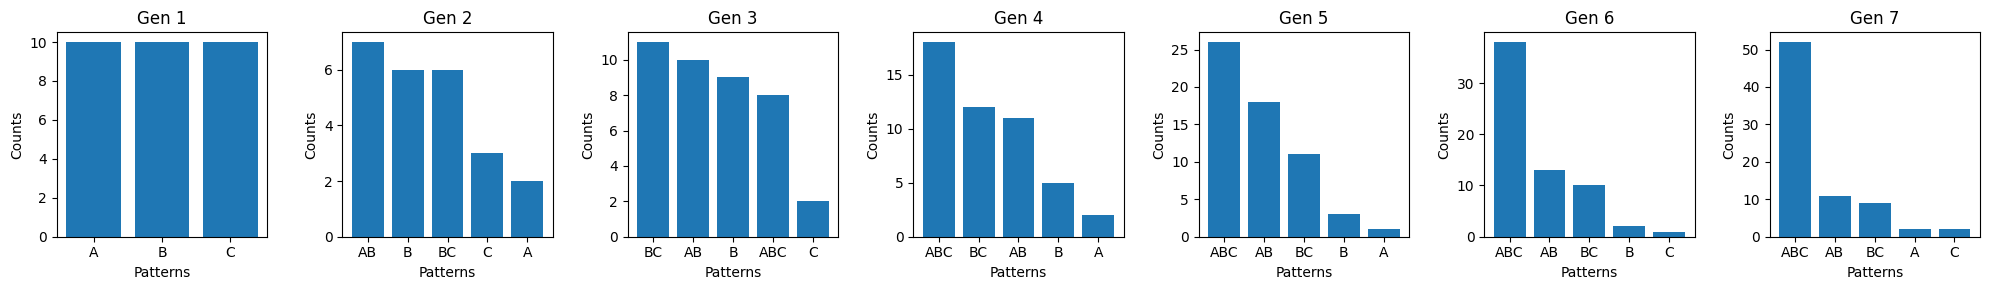
\includegraphics[width=13cm]{pat_1}
    \caption{ABC population histograms}
    \label{fig:pat_1}
\end{figure}

Where is Maxwell's demon hiding in this example, driving it towards a low-entropy state? The answer lies in the roulette wheel. Compounds that persist longer have more chances to interact. As their frequency in the population grows, their chances to interact grow even more. In Evolutionary Dynamics, this is called fitness-proportionate selection or roulette wheel selection.

\section{System Description and Dynamics}
In the more general case, denote the population of elements as:
\[
E = \{A, B, C, \dots\}.
\]
Each element \( X \) has a frequency \( f_X \), such that:
\[
\sum_{X \in E} f_X = 1.
\]

Pairs (or higher-order combinations) of elements can form compounds \( C_{XY}, C_{XYZ}, \dots \), with stability \( S(C) \) as a defining property. Stability \( S(C) \) measures how long the compound persists before dissociation. At each generation, elements interact, forming compounds with probabilities influenced by their frequencies. Define the fitness \( F(C) \) of a compound as proportional to its stability \( S(C) \):
\[
F(C) = S(C).
\]
Stable compounds persist longer and contribute more to the next generation's composition by dissociating into their constituent elements. The probability of forming a compound \( C_{XY} \) is proportional to:
\[
P(C_{XY}) \propto f_X \cdot f_Y \cdot g(C_{XY}),
\]
where \( g(C) \) is a function reflecting constraints such as geometry or energy barriers. More stable compounds contribute their elements back into the system with higher weights when they dissociate, biasing frequencies toward constituents of stable compounds. The frequency \( f_X^{(t+1)} \) at generation \( t+1 \) is updated as:
\begin{equation}
\label{eq1}
f_X^{(t+1)} = \frac{\sum_{C \ni X} F(C) \cdot P(C)}{\sum_{X'} \sum_{C \ni X'} F(C) \cdot P(C)},
\end{equation}
where \( P(C) \) is the probability of forming \( C \) in the previous generation. Over time, elements involved in forming more stable compounds \( (C_{XY}, C_{XYZ}, \dots) \) will increase in frequency. Elements with initially low frequencies may be outcompeted if they fail to form stable compounds. The system self-organizes toward a distribution of elements and compounds that maximizes overall stability.

Think of \( f_X \) as the relative "size" of \( X \)'s slot on the roulette wheel.
At each generation, higher \( f_X \) increases the likelihood of \( X \)'s participation in compounds. Fitness \( F(C) \) amplifies the impact of stable compounds, effectively "rigging" the wheel in favor of elements contributing to stability.

If \( F(C) \) and \( g(C) \) are constant, the system may converge to a stationary distribution \( f_X^* \), biased toward elements forming the most stable compounds. Initially random distributions \( f_X^{(0)} \) will evolve, reducing entropy as stable configurations dominate. The system exhibits a weak form of natural selection, where fitness is defined as stability rather than reproductive success.

In this case, the system’s fitness function is stability or persistence, which acts as a filter for preserving certain compounds and their constituent elements. Stability preferences impose a constraint on the system, reducing randomness. Elements forming stable compounds are selected for. Their frequencies increase, encoding knowledge about which interactions are favorable. In effect, the system learns and retains information about the stability landscape, evolving toward configurations with higher stability and the population becomes more ordered, reflecting lower entropy (negentropy). The Shannon entropy \( H \) at generation \( t \) is defined as:
\[
H^{(t)} = -\sum_{X \in E} f_X^{(t)} \log f_X^{(t)}.
\]
This measures the uncertainty or disorder in the system at generation \( t \). As the system evolves, the frequencies \( f_X^{(t)} \) are updated according to equation \eqref{eq1}. The evolution is biased toward elements involved in stable compounds, causing increased frequencies for elements in stable compounds, and reduced frequencies for elements in less stable or rarely formed compounds. This redistribution reduces entropy because high-probability elements dominate, concentrating the distribution, while low-probability elements contribute less, shrinking the uncertainty.

\subsection{Importance of Regeneration in Symbolic Systems}

\subsubsection{Avoiding Extinction in Population Dynamics}

In the absence of regeneration, the symbolic population tends to rapidly decline as base elements are consumed during interactions to form compounds. This creates a depletion cascade, where:
\begin{enumerate}
    \item Base elements \( X \in \{A, B, C, \ldots\} \) are continuously removed from the population as they participate in forming compounds \( C = AB, ABC, \ldots \).
    \item Compounds themselves decay over time, further reducing the population size without replenishing the base elements.
    \item Resource and energy constraints exacerbate this decline, as compounds fail to persist and contribute back to the system.
\end{enumerate}

Without an external mechanism to regenerate base elements, the system ultimately collapses, leading to extinction of the population. Regeneration is thus essential for sustaining the system across generations, ensuring a steady supply of base elements for ongoing interactions and compound formation.

\subsubsection{Physical Interpretation of Regeneration}

In physical systems, the regeneration of base symbols can be interpreted as the replenishment of fundamental building blocks through natural processes. Examples include:
\begin{itemize}
    \item \textbf{Atomic Systems}: Atoms or ions participating in chemical reactions can be regenerated by environmental processes such as diffusion or external inputs of reactive species.
    \item \textbf{Subatomic Particles}: Electrons in plasma systems can be regenerated through ionization or recombination processes, maintaining the particle population.
    \item \textbf{Energy Redistribution}: In ecosystems, energy flows from sunlight or chemical gradients provide the means for regenerating fundamental nutrients and resources.
\end{itemize}

In abstract systems, regeneration might represent:
\begin{itemize}
    \item \textbf{Data Initialization}: Reintroduction of lost or unused data elements to maintain diversity in computational systems.
    \item \textbf{Symbolic Restoration}: Replenishing foundational elements in symbolic or linguistic systems to sustain iterative processes.
\end{itemize}

\subsubsection{Regeneration in the Model}

To capture these dynamics, the symbolic framework includes a regeneration rate \( r_X \) for each base element \( X \), expressed as:
\begin{equation}
r_X(t+1) = r_X(t) + \rho_{\text{external}},
\end{equation}
where \( \rho_{\text{external}} \) is the external regeneration input per generation. This ensures a steady influx of base elements, enabling:
\begin{enumerate}
    \item \textbf{System Sustainability}: Preventing population collapse by replenishing consumed elements.
    \item \textbf{Dynamic Balance}: Allowing interactions to continue by maintaining a sufficient pool of base elements.
    \item \textbf{Pattern Evolution}: Supporting the emergence of stable patterns by providing the raw materials for compound formation.
\end{enumerate}


\subsection{Catalysis}

Other fitness criteria could also create frequency imbalances and drive the emergence of order and dominance in populations. These criteria depend on the specific system but share the common feature of amplifying certain elements or compounds based on measurable properties. Catalysis is one such example. Let's explore a system where \( A \) interacts with \( B \) to form a compound \( C_{AB} \), but this interaction occurs only in the presence of a catalyst \( D \). The catalyst \( D \) is not consumed or altered during the interaction, yet it influences the system's dynamics by facilitating specific reactions. We aim to show that this setup creates selection pressure for \( D \) to persist due to its role in enabling the formation of stable compounds. In this case, the catalyst \( D \) facilitates the reaction by increasing its likelihood:
\[
P(A + B \to C_{AB} \mid D) \propto f_A \cdot f_B \cdot f_D.
\]

The presence of \( D \) influences the formation rate of \( C_{AB} \), indirectly affecting the frequencies of \( A, B, \) and \( D \) through the dissociation of \( C_{AB} \):
\begin{align*}
f_A^{(t+1)} &= f_A^{(t)} + \alpha \cdot F(C_{AB}) \cdot f_A^{(t)} \cdot f_B^{(t)} \cdot f_D^{(t)}, \\
f_B^{(t+1)} &= f_B^{(t)} + \alpha \cdot F(C_{AB}) \cdot f_A^{(t)} \cdot f_B^{(t)} \cdot f_D^{(t)}, \\
f_D^{(t+1)} &= f_D^{(t)} + \beta \cdot F(C_{AB}) \cdot f_A^{(t)} \cdot f_B^{(t)} \cdot f_D^{(t)}.
\end{align*}
where \( \alpha \) is the proportionality constant for reactants, and \( \beta \) is the contribution of \( D \) from catalysis.

Although \( D \) is not consumed in the reaction, its presence enables the formation of \( C_{AB} \), which dissociates and contributes to \( f_D \):
\[
f_D^{(t+1)} > f_D^{(t)} \quad \text{if } f_A \cdot f_B \cdot F(C_{AB}) > \text{threshold}.
\]
This creates selection pressure for \( D \), as its persistence increases the system's ability to form stable \( C_{AB} \), reinforcing its own frequency. The catalyst \( D \) benefits indirectly, as its presence enables reactions that increase the overall fitness of the system, and the resulting higher fitness compounds contribute to \( f_D \), creating a positive feedback loop. Over successive generations, elements \( A \) and \( B \) rely on \( D \) to form \( C_{AB} \) and the system selects for \( D \), even if its own stability is low, because it amplifies the system's stability.

This catalytic framework demonstrates how an element that facilitates reactions, without directly participating in the products, can experience selection pressure. The persistence of \( D \) arises from its indirect contribution to the system's fitness by enabling the formation of stable compounds which decrease the system's entropy.

\section{Mixing Two Populations: Opportunities for Crossover and Symbiosis}

Mixing two previously separate populations introduces new interaction dynamics, enabling the formation of new stable combinations of unique compounds arising from cross-population interactions, as well as new catalytic elements enhancing reaction rates, creating pathways for more stable patterns than existed in either population individually.

Imagine two such populations: \( E_1 = \{A_1, B_1, C_1, \dots\} \), \( E_2 = \{A_2, B_2, C_2, \dots\} \) each at a different stage in its evolution. Within each population there will be compounds such as \( C_{A_1B_1} \) and \( C_{A_2B_2} \), but now there are opportunities to form new compounds across both populations, e.g., \( C_{A_1B_2}, C_{A_2B_1} \), which were previously impossible. These compounds could be more stable than any of the compounds in either population, which would create new imbalances that further reduce the entropy of the combined population. We can call this crossover, as it closely resembles genetic crossover in biotic evolution.

Furthermore, catalysts in \( E_1 \) may stabilize reactions in \( E_2 \) and vice versa, introducing symbiotic dynamics:
\[
P(A_1 + B_2 \to C_{A_1B_2} \mid D_1) \propto f_{A_1} \cdot f_{B_2} \cdot f_{D_1}.
\]

Cross-population interactions increase the diversity of compounds. For example:
\[
F(C_{A_1B_2}) = S(C_{A_1B_2}) \quad \text{and} \quad F(C_{A_2B_1}) = S(C_{A_2B_1}),
\]
where \( S(C) \) measures the stability of new compounds. These compounds contribute to the fitness landscape of both populations. Catalysts from one population (\( D_1 \)) may enable reactions in the other population (\( E_2 \)):
\[
P(A_2 + B_2 \to C_{A_2B_2} \mid D_1) \propto f_{A_2} \cdot f_{B_2} \cdot f_{D_1}.
\]
Such symbiotic relationships increase the persistence of \( D_1 \) and \( D_2 \), enhancing the overall stability of the mixed population.

Cross-population compounds and catalytic symbiosis introduce new feedback loops: the formation of \( C_{A_1B_2} \) increases \( f_{A_1} \) and \( f_{B_2} \), and the enhanced stability of \( C_{A_2B_1} \) reinforces the presence of \( A_2 \) and \( B_1 \).

\section{Analogy to Evolutionary Mechanisms}

\subsection*{Crossover in Genetics}
The formation of cross-population compounds parallels genetic crossover in biological systems, where recombination generates new traits.

\subsection*{Symbiosis in Ecosystems}
Catalytic interactions between populations resemble symbiotic relationships in ecosystems, where mutual benefits drive stability and persistence.

\section{Mathematical Properties}

\subsection*{Stationary Distribution}
If \( F(C) \) and \( g(C) \) are constant, the mixed system converges to a stationary distribution:
\[
f_X^* \quad \text{biased toward elements forming stable cross-population compounds.}
\]

\subsection*{Entropy Reduction}
The mixing of populations initially increases diversity, raising entropy. However, as stable compounds dominate, entropy decreases:
\[
H^{(t+1)} < H^{(t)}.
\]

\subsection*{Enhanced Stability}
Mixed populations can achieve greater stability than isolated populations:
\[
\max(S(C_{XY})) \text{ in mixed populations} > \max(S(C_{XY})) \text{ in isolated populations.}
\]

\section{Introduction}

Emergent phenomena in complex systems often defy simple bottom-up explanations, as the interplay between local interactions and global feedback can generate hierarchical structures and persistent patterns~\cite{anderson1972more}. This paper explores a framework for the emergence of stability in symbolic systems, where probabilistic interactions, regeneration dynamics, and feedback loops drive the evolution of patterns. Using simulations inspired by prebiotic evolution and resource-constrained environments, we demonstrate the principles of feedback-driven stability and discuss implications for Bayesian reasoning, top-down causality, and the evolution of information.

\section{Theoretical Framework}

\subsection{Feedback Dynamics in Symbolic Systems}

Let a system consist of a population of elements \( E = \{A, B, C, \ldots\} \), where each element \( X \in E \) has a frequency \( p_X \) and a regeneration rate \( r_X \). Pairs (or higher-order combinations) of elements form compounds \( C = AB, ABC, \ldots \), characterized by their stability \( S(C) \).

\subsubsection{Regeneration Feedback Loop}

The regeneration rate \( r_X \) evolves based on the frequency of compounds containing \( X \):
\begin{equation}
r_X(t+1) = r_X(t) + \alpha \sum_{C \ni X} p(C),
\end{equation}
where \( \alpha \) is the feedback strength and \( p(C) \) is the frequency of compound \( C \). This feedback loop creates a self-reinforcing mechanism where elements contributing to stable patterns are regenerated more frequently.

\subsubsection{Interaction Probabilities}

Interactions between elements and compounds are governed by their regeneration rates and stability:
\begin{equation}
P(C = AB) \propto r_A \cdot r_B \cdot (1 + \beta \cdot S(C)),
\end{equation}
where \( \beta \) biases interactions toward stable compounds.

\subsubsection{Resource Allocation and Persistence}

Resources are allocated preferentially to stable compounds:
\begin{equation}
R(C) = \frac{S(C)}{\sum_{C'} S(C')},
\end{equation}
ensuring that persistent compounds dominate over time.

\section{Simulation Results}

We implemented the framework in a Python simulation, using symbolic populations with base elements \( A, B, C, X, Y, Z \). Key parameters include regeneration rates, interaction probabilities, and resource constraints. 

\subsection{Frequency Dynamics and Stability Emergence}

Simulations showed that stable patterns emerged as a result of feedback loops. Dominant compounds persisted across generations, and their constituent elements were regenerated at higher rates. Adjustments, such as increasing the interaction bias toward stable compounds or reducing the regeneration rate of less frequent elements, amplified these effects.

\subsection{Bayesian Reasoning in Population Dynamics}

The frequency dynamics between generations can be interpreted through Bayesian reasoning:
\begin{equation}
p(C|t+1) \propto p(C|t) \cdot \text{Fitness}(C),
\end{equation}
where fitness is proportional to stability \( S(C) \). This reflects a process where each generation updates its distribution of patterns based on environmental feedback, analogous to Bayesian inference.

\subsection{Top-Down and Bottom-Up Causality}

The framework illustrates how top-down causality arises in emergent systems. Stable patterns influence the regeneration rates of their constituent elements, thereby shaping the local interaction rules. This feedback loop creates a co-dependence between top-down (pattern-level) and bottom-up (element-level) dynamics, challenging reductionist views that prioritize microstates over macrostates~\cite{laughlin2000different}.

\section{Discussion}

\subsection{Implications for Biological and Chemical Systems}

The principles of feedback-driven stability have parallels in biological evolution and prebiotic chemistry. For example, autocatalytic cycles in chemical networks exhibit similar dynamics, where stability emerges through self-reinforcing interactions~\cite{kauffman1993origins}.

\subsection{Universal Principles of Emergence}

The framework suggests that emergent stability is a universal property of systems with probabilistic interactions, resource constraints, and feedback loops. This aligns with theories of self-organized criticality, where local rules generate global order~\cite{bak1996how}.

\subsection{Bayesian and Mystical Interpretations}

The Bayesian perspective on frequency dynamics connects mathematical reasoning to the evolution of information. Interestingly, mystical traditions such as Kabbalah and certain Indian philosophies resonate with the notion of transcendental principles guiding physical systems. However, our findings suggest that these principles are co-dependent on the dynamics of the systems they govern.

\section{Conclusion}

Feedback-driven stability offers a unifying framework for understanding pattern formation in emergent systems. By combining Bayesian reasoning with insights into top-down and bottom-up causality, this approach provides a new lens to study the evolution of information across diverse domains.

\section{Predator-Prey Dynamics in Symbolic Systems}

\subsection{Mapping Symbolic Interactions to Predator-Prey Models}

The dynamics of the symbolic system can be conceptualized using predator-prey models, where the base elements act as "prey," and the compounds they form act as "predators." The interplay between regeneration rates of base symbols and the stability of compounds creates a feedback loop analogous to classical predator-prey relationships.

In this analogy:
\begin{itemize}
    \item \textbf{Base elements} (\( A, B, C, \ldots \)) represent the prey, which are replenished through regeneration.
    \item \textbf{Compounds} (\( AB, ABC, \ldots \)) represent the predators, which consume base elements during interactions and persist based on their stability.
\end{itemize}

\subsection{Differential Equations for Predator-Prey Dynamics}

The dynamics can be expressed through a modified Lotka-Volterra system, where the populations of base elements (\( N_X \)) and compounds (\( N_C \)) evolve as:
\begin{align}
\frac{dN_X}{dt} &= r_X \cdot N_X - \sum_C P(C) \cdot N_X, \\
\frac{dN_C}{dt} &= \beta \cdot P(C) \cdot N_X - \delta \cdot N_C,
\end{align}
where:
\begin{itemize}
    \item \( r_X \): Regeneration rate of the base element \( X \) (prey).
    \item \( P(C) \): Probability of forming compound \( C \) (predator).
    \item \( \beta \): Rate of compound formation (predator growth rate).
    \item \( \delta \): Decay rate of compounds (predator mortality rate).
\end{itemize}

These equations describe a dynamic balance:
\begin{enumerate}
    \item Base elements are replenished at a rate proportional to \( r_X \), but are depleted by interactions forming compounds.
    \item Compounds grow in population as they consume base elements but decay over time due to resource competition and energy constraints.
\end{enumerate}

\subsection{Emergent Stability from Predator-Prey Feedback}

The predator-prey model inherently incorporates feedback:
\begin{itemize}
    \item \textbf{Prey Regulation}: The regeneration rates \( r_X \) dynamically adjust based on the presence of compounds, reflecting a feedback loop that maintains the population of base elements.
    \item \textbf{Predator Reinforcement}: Persistent compounds act as "successful predators," increasing the regeneration of their constituent base elements and stabilizing their own presence.
\end{itemize}

This dynamic leads to emergent stability, where certain compounds dominate due to their ability to balance resource consumption (prey depletion) and persistence (predator survival).

\subsection{Comparison to Classical Predator-Prey Systems}

Unlike traditional predator-prey models, this system includes:
\begin{itemize}
    \item \textbf{Feedback in Regeneration}: The regeneration rates \( r_X \) are influenced by the compounds they help form, creating a self-reinforcing loop absent in classical models.
    \item \textbf{Stability Bias}: Compounds with higher stability (\( S(C) \)) disproportionately affect the regeneration and interaction dynamics, skewing the system toward emergent patterns.
    \item \textbf{Multi-Prey and Multi-Predator Interactions}: Compounds can act as predators that consume multiple base elements (prey), while also being prey for higher-order interactions.
\end{itemize}

\subsection{Implications for Emergent Patterns}

The predator-prey analogy highlights:
\begin{enumerate}
    \item \textbf{Resource Constraints}: Persistent compounds stabilize by balancing consumption and regeneration, ensuring long-term survival in a resource-limited environment.
    \item \textbf{Hierarchical Emergence}: The interplay between base elements and compounds creates a hierarchical system, with dominant compounds shaping the population dynamics of their constituent elements.
    \item \textbf{Universal Applicability}: These principles extend beyond symbolic systems, providing insights into ecological networks, chemical reaction systems, and evolutionary dynamics.
\end{enumerate}

The predator-prey perspective complements the Bayesian and top-down causality interpretations, offering an alternative lens to understand the co-dependence of local interactions and global stability.

\section{Incorporating Resources and Energy into Symbolic Systems}

\subsection{Energy as a Limiting Factor in Interactions}

In real-world systems, interactions between elements and the persistence of patterns are often constrained by the availability of energy. To incorporate this into the symbolic framework, we introduce an explicit energy model, where:
\begin{itemize}
    \item \textbf{Total Energy}: The system starts with an initial energy pool \( E(t) \), which is replenished at each generation by an external energy source.
    \item \textbf{Energy for Interactions}: Each interaction consumes a fixed amount of energy proportional to the size of the compound formed.
    \item \textbf{Energy Recycling}: Decaying compounds release a fraction of their energy back into the system, reflecting energy recycling dynamics.
\end{itemize}

\subsection{Mathematical Model for Energy Dynamics}

The energy dynamics are modeled as follows:
\begin{align}
E(t+1) &= E(t) + \epsilon_{\text{replenish}} - \epsilon_{\text{interactions}} + \epsilon_{\text{recycled}}, \\
\epsilon_{\text{interactions}} &= \sum_{i=1}^{N} \epsilon_{\text{cost}}(C_i), \\
\epsilon_{\text{recycled}} &= \sum_{j=1}^{M} \gamma \cdot S(C_j),
\end{align}
where:
\begin{itemize}
    \item \( E(t) \): Total energy at generation \( t \).
    \item \( \epsilon_{\text{replenish}} \): Energy added externally to the system at each generation.
    \item \( \epsilon_{\text{interactions}} \): Energy consumed during interactions.
    \item \( \epsilon_{\text{cost}}(C_i) \): Energy cost of forming compound \( C_i \), proportional to its size or complexity.
    \item \( \epsilon_{\text{recycled}} \): Energy recycled from decaying compounds.
    \item \( \gamma \): Fraction of stability \( S(C_j) \) recycled into usable energy.
\end{itemize}

\subsection{Resource Constraints on Regeneration}

In addition to energy, resources are treated as a separate pool \( R(t) \), representing the raw materials needed to regenerate base elements and form compounds:
\begin{align}
R(t+1) &= R(t) + \rho_{\text{replenish}} - \rho_{\text{consumed}}, \\
\rho_{\text{consumed}} &= \sum_{C} \lambda \cdot \text{size}(C),
\end{align}
where:
\begin{itemize}
    \item \( R(t) \): Total resources at generation \( t \).
    \item \( \rho_{\text{replenish}} \): Resources replenished at each generation.
    \item \( \rho_{\text{consumed}} \): Resources consumed during interactions, proportional to compound size.
    \item \( \lambda \): Resource cost per unit of compound size.
\end{itemize}

\subsection{Energy and Resource Allocation for Patterns}

Energy and resources are allocated based on compound stability \( S(C) \):
\begin{align}
\text{Energy Share } \epsilon(C) &= \frac{S(C)}{\sum_{C'} S(C')}, \\
\text{Resource Share } \rho(C) &= \frac{S(C)}{\sum_{C'} S(C')}.
\end{align}
Compounds with higher stability are allocated a larger share, promoting their persistence and dominance in the population.

\subsection{Emergent Dynamics with Energy and Resources}

Adding energy and resources introduces new constraints and opportunities:
\begin{enumerate}
    \item \textbf{Resource Competition}: Compounds compete for limited resources and energy, favoring the most stable patterns.
    \item \textbf{Energy Recycling}: The recycling of energy from decaying compounds creates a feedback loop, ensuring long-term sustainability of the system.
    \item \textbf{Persistence of Stable Patterns}: Stability directly influences energy and resource allocation, reinforcing the dominance of persistent patterns.
\end{enumerate}

\subsection{Comparison to Real-World Systems}

This model mirrors real-world phenomena:
\begin{itemize}
    \item \textbf{Biological Systems}: Energy and nutrient cycles in ecosystems are analogous to energy recycling and resource replenishment in the model.
    \item \textbf{Chemical Systems}: Reaction networks depend on the availability of energy to form and break bonds, analogous to the energy costs of forming compounds.
    \item \textbf{Information Systems}: Computational processes constrained by energy and resource availability exhibit similar dynamics, with stable patterns corresponding to persistent solutions.
\end{itemize}

\subsection{Implications for Stability and Complexity}

The incorporation of energy and resources enhances the framework by:
\begin{enumerate}
    \item Providing a mechanism to regulate the balance between base elements and compounds.
    \item Highlighting the role of external inputs in driving complexity and stability.
    \item Offering insights into how energy constraints shape emergent behavior in both physical and abstract systems.
\end{enumerate}




%%%%%%%%%%%%%%%%%%%%%%%%%%%%%%%%%%%%%%%%%%
\section{Materials and Methods}

Materials and Methods should be described with sufficient details to allow others to replicate and build on published results. Please note that publication of your manuscript implicates that you must make all materials, data, computer code, and protocols associated with the publication available to readers. Please disclose at the submission stage any restrictions on the availability of materials or information. New methods and protocols should be described in detail while well-established methods can be briefly described and appropriately cited.

Research manuscripts reporting large datasets that are deposited in a publicly avail-able database should specify where the data have been deposited and provide the relevant accession numbers. If the accession numbers have not yet been obtained at the time of submission, please state that they will be provided during review. They must be provided prior to publication.

Interventionary studies involving animals or humans, and other studies require ethical approval must list the authority that provided approval and the corresponding ethical approval code.
\begin{quote}
This is an example of a quote.
\end{quote}

%%%%%%%%%%%%%%%%%%%%%%%%%%%%%%%%%%%%%%%%%%
\section{Results}

This section may be divided by subheadings. It should provide a concise and precise description of the experimental results, their interpretation as well as the experimental conclusions that can be drawn.
\subsection{Subsection}
\subsubsection{Subsubsection}

Bulleted lists look like this:
\begin{itemize}
\item	First bullet;
\item	Second bullet;
\item	Third bullet.
\end{itemize}

Numbered lists can be added as follows:
\begin{enumerate}
\item	First item; 
\item	Second item;
\item	Third item.
\end{enumerate}

The text continues here. 

\subsection{Figures, Tables and Schemes}

All figures and tables should be cited in the main text as Figure~\ref{fig1}, Table~\ref{tab1}, etc.

\begin{figure}[H]

\includegraphics[width=10.5 cm]{Definitions/logo-mdpi}
\caption{This is a figure. Schemes follow the same formatting. If there are multiple panels, they should be listed as: (\textbf{a}) Description of what is contained in the first panel. (\textbf{b}) Description of what is contained in the second panel. Figures should be placed in the main text near to the first time they are cited. A caption on a single line should be centered.\label{fig1}}
\end{figure}   
\unskip

\begin{table}[H] 
\caption{This is a table caption. Tables should be placed in the main text near to the first time they are~cited.\label{tab1}}
%\newcolumntype{C}{>{\centering\arraybackslash}X}
\begin{tabularx}{\textwidth}{CCC}
\toprule
\textbf{Title 1}	& \textbf{Title 2}	& \textbf{Title 3}\\
\midrule
Entry 1		& Data			& Data\\
Entry 2		& Data			& Data \textsuperscript{1}\\
\bottomrule
\end{tabularx}
\noindent{\footnotesize{\textsuperscript{1} Tables may have a footer.}}
\end{table}

The text continues here (Figure~\ref{fig2} and Table~\ref{tab2}).

% Example of a figure that spans the whole page width. The same concept works for tables, too.
\begin{figure}[H]
\begin{adjustwidth}{-\extralength}{0cm}
\centering

\includegraphics[width=15.5cm]{Definitions/logo-mdpi}
\end{adjustwidth}
\caption{This is a wide figure.\label{fig2}}
\end{figure}  

\begin{table}[H]
\caption{This is a wide table.\label{tab2}}
	\begin{adjustwidth}{-\extralength}{0cm}
%		\newcolumntype{C}{>{\centering\arraybackslash}X}
		\begin{tabularx}{\fulllength}{CCCC}
			\toprule
			\textbf{Title 1}	& \textbf{Title 2}	& \textbf{Title 3}     & \textbf{Title 4}\\
			\midrule
\multirow[m]{3}{*}{Entry 1 *}	& Data			& Data			& Data\\
			  	                   & Data			& Data			& Data\\
			             	      & Data			& Data			& Data\\
                   \midrule
\multirow[m]{3}{*}{Entry 2}    & Data			& Data			& Data\\
			  	                  & Data			& Data			& Data\\
			             	     & Data			& Data			& Data\\
                   \midrule
\multirow[m]{3}{*}{Entry 3}    & Data			& Data			& Data\\
			  	                 & Data			& Data			& Data\\
			             	    & Data			& Data			& Data\\
                  \midrule
\multirow[m]{3}{*}{Entry 4}   & Data			& Data			& Data\\
			  	                 & Data			& Data			& Data\\
			             	    & Data			& Data			& Data\\
			\bottomrule
		\end{tabularx}
	\end{adjustwidth}
	\noindent{\footnotesize{* Tables may have a footer.}}
\end{table}

%\begin{listing}[H]
%\caption{Title of the listing}
%\rule{\columnwidth}{1pt}
%\raggedright Text of the listing. In font size footnotesize, small, or normalsize. Preferred format: left aligned and single spaced. Preferred border format: top border line and bottom border line.
%\rule{\columnwidth}{1pt}
%\end{listing}

Text.

Text.

\subsection{Formatting of Mathematical Components}

This is the example 1 of equation:
\begin{linenomath}
\begin{equation}
a = 1,
\end{equation}
\end{linenomath}
the text following an equation need not be a new paragraph. Please punctuate equations as regular text.
%% If the documentclass option "submit" is chosen, please insert a blank line before and after any math environment (equation and eqnarray environments). This ensures correct linenumbering. The blank line should be removed when the documentclass option is changed to "accept" because the text following an equation should not be a new paragraph.

This is the example 2 of equation:
\begin{adjustwidth}{-\extralength}{0cm}
\begin{equation}
a = b + c + d + e + f + g + h + i + j + k + l + m + n + o + p + q + r + s + t + u + v + w + x + y + z
\end{equation}
\end{adjustwidth}

% Example of a page in landscape format (with table and table footnote).
%\startlandscape
%\begin{table}[H] %% Table in wide page
%\caption{This is a very wide table.\label{tab3}}
%	\begin{tabularx}{\textwidth}{CCCC}
%		\toprule
%		\textbf{Title 1}	& \textbf{Title 2}	& \textbf{Title 3}	& \textbf{Title 4}\\
%		\midrule
%		Entry 1		& Data			& Data			& This cell has some longer content that runs over two lines.\\
%		Entry 2		& Data			& Data			& Data\textsuperscript{1}\\
%		\bottomrule
%	\end{tabularx}
%	\begin{adjustwidth}{+\extralength}{0cm}
%		\noindent\footnotesize{\textsuperscript{1} This is a table footnote.}
%	\end{adjustwidth}
%\end{table}
%\finishlandscape


Please punctuate equations as regular text. Theorem-type environments (including propositions, lemmas, corollaries etc.) can be formatted as follows:
%% Example of a theorem:
\begin{Theorem}
Example text of a theorem.
\end{Theorem}

The text continues here. Proofs must be formatted as follows:

%% Example of a proof:
\begin{proof}[Proof of Theorem 1]
Text of the proof. Note that the phrase ``of Theorem 1'' is optional if it is clear which theorem is being referred to.
\end{proof}
The text continues here.

%%%%%%%%%%%%%%%%%%%%%%%%%%%%%%%%%%%%%%%%%%
\section{Discussion}

Authors should discuss the results and how they can be interpreted from the perspective of previous studies and of the working hypotheses. The findings and their implications should be discussed in the broadest context possible. Future research directions may also be highlighted.

%%%%%%%%%%%%%%%%%%%%%%%%%%%%%%%%%%%%%%%%%%
\section{Conclusions}

This section is not mandatory, but can be added to the manuscript if the discussion is unusually long or complex.

%%%%%%%%%%%%%%%%%%%%%%%%%%%%%%%%%%%%%%%%%%
\section{Patents}

This section is not mandatory, but may be added if there are patents resulting from the work reported in this manuscript.

%%%%%%%%%%%%%%%%%%%%%%%%%%%%%%%%%%%%%%%%%%
\vspace{6pt} 

%%%%%%%%%%%%%%%%%%%%%%%%%%%%%%%%%%%%%%%%%%
%% optional
%\supplementary{The following supporting information can be downloaded at:  \linksupplementary{s1}, Figure S1: title; Table S1: title; Video S1: title.}

% Only for journal Methods and Protocols:
% If you wish to submit a video article, please do so with any other supplementary material.
% \supplementary{The following supporting information can be downloaded at: \linksupplementary{s1}, Figure S1: title; Table S1: title; Video S1: title. A supporting video article is available at doi: link.}

% Only for journal Hardware:
% If you wish to submit a video article, please do so with any other supplementary material.
% \supplementary{The following supporting information can be downloaded at: \linksupplementary{s1}, Figure S1: title; Table S1: title; Video S1: title.\vspace{6pt}\\
%\begin{tabularx}{\textwidth}{lll}
%\toprule
%\textbf{Name} & \textbf{Type} & \textbf{Description} \\
%\midrule
%S1 & Python script (.py) & Script of python source code used in XX \\
%S2 & Text (.txt) & Script of modelling code used to make Figure X \\
%S3 & Text (.txt) & Raw data from experiment X \\
%S4 & Video (.mp4) & Video demonstrating the hardware in use \\
%... & ... & ... \\
%\bottomrule
%\end{tabularx}
%}

%%%%%%%%%%%%%%%%%%%%%%%%%%%%%%%%%%%%%%%%%%
\authorcontributions{For research articles with several authors, a short paragraph specifying their individual contributions must be provided. The following statements should be used ``Conceptualization, X.X. and Y.Y.; methodology, X.X.; software, X.X.; validation, X.X., Y.Y. and Z.Z.; formal analysis, X.X.; investigation, X.X.; resources, X.X.; data curation, X.X.; writing---original draft preparation, X.X.; writing---review and editing, X.X.; visualization, X.X.; supervision, X.X.; project administration, X.X.; funding acquisition, Y.Y. All authors have read and agreed to the published version of the manuscript.'', please turn to the  \href{http://img.mdpi.org/data/contributor-role-instruction.pdf}{CRediT taxonomy} for the term explanation. Authorship must be limited to those who have contributed substantially to the work~reported.}

\funding{Please add: ``This research received no external funding'' or ``This research was funded by NAME OF FUNDER grant number XXX.'' and  and ``The APC was funded by XXX''. Check carefully that the details given are accurate and use the standard spelling of funding agency names at \url{https://search.crossref.org/funding}, any errors may affect your future funding.}

\institutionalreview{In this section, you should add the Institutional Review Board Statement and approval number, if relevant to your study. You might choose to exclude this statement if the study did not require ethical approval. Please note that the Editorial Office might ask you for further information. Please add “The study was conducted in accordance with the Declaration of Helsinki, and approved by the Institutional Review Board (or Ethics Committee) of NAME OF INSTITUTE (protocol code XXX and date of approval).” for studies involving humans. OR “The animal study protocol was approved by the Institutional Review Board (or Ethics Committee) of NAME OF INSTITUTE (protocol code XXX and date of approval).” for studies involving animals. OR “Ethical review and approval were waived for this study due to REASON (please provide a detailed justification).” OR “Not applicable” for studies not involving humans or animals.}

\informedconsent{Any research article describing a study involving humans should contain this statement. Please add ``Informed consent was obtained from all subjects involved in the study.'' OR ``Patient consent was waived due to REASON (please provide a detailed justification).'' OR ``Not applicable'' for studies not involving humans. You might also choose to exclude this statement if the study did not involve humans.

Written informed consent for publication must be obtained from participating patients who can be identified (including by the patients themselves). Please state ``Written informed consent has been obtained from the patient(s) to publish this paper'' if applicable.}

\dataavailability{We encourage all authors of articles published in MDPI journals to share their research data. In this section, please provide details regarding where data supporting reported results can be found, including links to publicly archived datasets analyzed or generated during the study. Where no new data were created, or where data is unavailable due to privacy or ethical restrictions, a statement is still required. Suggested Data Availability Statements are available in section ``MDPI Research Data Policies'' at \url{https://www.mdpi.com/ethics}.} 

% Only for journal Nursing Reports
%\publicinvolvement{Please describe how the public (patients, consumers, carers) were involved in the research. Consider reporting against the GRIPP2 (Guidance for Reporting Involvement of Patients and the Public) checklist. If the public were not involved in any aspect of the research add: ``No public involvement in any aspect of this research''.}

% Only for journal Nursing Reports
%\guidelinesstandards{Please add a statement indicating which reporting guideline was used when drafting the report. For example, ``This manuscript was drafted against the XXX (the full name of reporting guidelines and citation) for XXX (type of research) research''. A complete list of reporting guidelines can be accessed via the equator network: \url{https://www.equator-network.org/}.}

% Only for journal Nursing Reports
%\useofartificialintelligence{Please describe in detail any and all uses of artificial intelligence (AI) or AI-assisted tools used in the preparation of the manuscript. This may include, but is not limited to, language translation, language editing and grammar, or generating text. Alternatively, please state that “AI or AI-assisted tools were not used in drafting any aspect of this manuscript”.}

\acknowledgments{In this section you can acknowledge any support given which is not covered by the author contribution or funding sections. This may include administrative and technical support, or donations in kind (e.g., materials used for experiments).}

\conflictsofinterest{Declare conflicts of interest or state ``The authors declare no conflicts of interest.'' Authors must identify and declare any personal circumstances or interest that may be perceived as inappropriately influencing the representation or interpretation of reported research results. Any role of the funders in the design of the study; in the collection, analyses or interpretation of data; in the writing of the manuscript; or in the decision to publish the results must be declared in this section. If there is no role, please state ``The funders had no role in the design of the study; in the collection, analyses, or interpretation of data; in the writing of the manuscript; or in the decision to publish the results''.} 

%%%%%%%%%%%%%%%%%%%%%%%%%%%%%%%%%%%%%%%%%%
%% Optional

%% Only for journal Encyclopedia
%\entrylink{The Link to this entry published on the encyclopedia platform.}

\abbreviations{Abbreviations}{
The following abbreviations are used in this manuscript:\\

\noindent 
\begin{tabular}{@{}ll}
MDPI & Multidisciplinary Digital Publishing Institute\\
DOAJ & Directory of open access journals\\
TLA & Three letter acronym\\
LD & Linear dichroism
\end{tabular}
}

%%%%%%%%%%%%%%%%%%%%%%%%%%%%%%%%%%%%%%%%%%
%% Optional
\appendixtitles{no} % Leave argument "no" if all appendix headings stay EMPTY (then no dot is printed after "Appendix A"). If the appendix sections contain a heading then change the argument to "yes".
\appendixstart
\appendix
\section[\appendixname~\thesection]{}
\subsection[\appendixname~\thesubsection]{}
The appendix is an optional section that can contain details and data supplemental to the main text---for example, explanations of experimental details that would disrupt the flow of the main text but nonetheless remain crucial to understanding and reproducing the research shown; figures of replicates for experiments of which representative data are shown in the main text can be added here if brief, or as Supplementary Data. Mathematical proofs of results not central to the paper can be added as an appendix.

\begin{table}[H] 
\caption{This is a table caption.\label{tab5}}
\newcolumntype{C}{>{\centering\arraybackslash}X}
\begin{tabularx}{\textwidth}{CCC}
\toprule
\textbf{Title 1}	& \textbf{Title 2}	& \textbf{Title 3}\\
\midrule
Entry 1		& Data			& Data\\
Entry 2		& Data			& Data\\
\bottomrule
\end{tabularx}
\end{table}

\section[\appendixname~\thesection]{}
All appendix sections must be cited in the main text. In the appendices, Figures, Tables, etc. should be labeled, starting with ``A''---e.g., Figure A1, Figure A2, etc.

%%%%%%%%%%%%%%%%%%%%%%%%%%%%%%%%%%%%%%%%%%
\begin{adjustwidth}{-\extralength}{0cm}
%\printendnotes[custom] % Un-comment to print a list of endnotes

\reftitle{References}

% Please provide either the correct journal abbreviation (e.g. according to the “List of Title Word Abbreviations” http://www.issn.org/services/online-services/access-to-the-ltwa/) or the full name of the journal.
% Citations and References in Supplementary files are permitted provided that they also appear in the reference list here. 

%=====================================
% References, variant A: external bibliography
%=====================================
%\bibliography{your_external_BibTeX_file}

%=====================================
% References, variant B: internal bibliography
%=====================================
\begin{thebibliography}{999}
% Reference 1
\bibitem[Author1(year)]{ref-journal}
Author~1, T. The title of the cited article. {\em Journal Abbreviation} {\bf 2008}, {\em 10}, 142--149.
% Reference 2
\bibitem[Author2(year)]{ref-book1}
Author~2, L. The title of the cited contribution. In {\em The Book Title}; Editor 1, F., Editor 2, A., Eds.; Publishing House: City, Country, 2007; pp. 32--58.
% Reference 3
\bibitem[Author3(year)]{ref-book2}
Author 1, A.; Author 2, B. \textit{Book Title}, 3rd ed.; Publisher: Publisher Location, Country, 2008; pp. 154--196.
% Reference 4
\bibitem[Author4(year)]{ref-unpublish}
Author 1, A.B.; Author 2, C. Title of Unpublished Work. \textit{Abbreviated Journal Name} year, \textit{phrase indicating stage of publication (submitted; accepted; in press)}.
% Reference 5
\bibitem[Author5(year)]{ref-communication}
Author 1, A.B. (University, City, State, Country); Author 2, C. (Institute, City, State, Country). Personal communication, 2012.
% Reference 6
\bibitem[Author6(year)]{ref-proceeding}
Author 1, A.B.; Author 2, C.D.; Author 3, E.F. Title of presentation. In Proceedings of the Name of the Conference, Location of Conference, Country, Date of Conference (Day Month Year); Abstract Number (optional), Pagination (optional).
% Reference 7
\bibitem[Author7(year)]{ref-thesis}
Author 1, A.B. Title of Thesis. Level of Thesis, Degree-Granting University, Location of University, Date of Completion.
% Reference 8
\bibitem[Author8(year)]{ref-url}
Title of Site. Available online: URL (accessed on Day Month Year).
\end{thebibliography}

% If authors have biography, please use the format below
%\section*{Short Biography of Authors}
%\bio
%{\raisebox{-0.35cm}{\includegraphics[width=3.5cm,height=5.3cm,clip,keepaspectratio]{Definitions/author1.pdf}}}
%{\textbf{Firstname Lastname} Biography of first author}
%
%\bio
%{\raisebox{-0.35cm}{\includegraphics[width=3.5cm,height=5.3cm,clip,keepaspectratio]{Definitions/author2.jpg}}}
%{\textbf{Firstname Lastname} Biography of second author}

% For the MDPI journals use author-date citation, please follow the formatting guidelines on http://www.mdpi.com/authors/references
% To cite two works by the same author: \citeauthor{ref-journal-1a} (\citeyear{ref-journal-1a}, \citeyear{ref-journal-1b}). This produces: Whittaker (1967, 1975)
% To cite two works by the same author with specific pages: \citeauthor{ref-journal-3a} (\citeyear{ref-journal-3a}, p. 328; \citeyear{ref-journal-3b}, p.475). This produces: Wong (1999, p. 328; 2000, p. 475)

%%%%%%%%%%%%%%%%%%%%%%%%%%%%%%%%%%%%%%%%%%
%% for journal Sci
%\reviewreports{\\
%Reviewer 1 comments and authors’ response\\
%Reviewer 2 comments and authors’ response\\
%Reviewer 3 comments and authors’ response
%}
%%%%%%%%%%%%%%%%%%%%%%%%%%%%%%%%%%%%%%%%%%
\PublishersNote{}
\end{adjustwidth}
\end{document}

